% !TeX program = lualatex
% ================================================================
% Polish Parallel Text Version of ShapeAndAveragesStarters
%
% Generated by the server using the following settings:
%
%   language            Polish (pol)
%   text direction      left to right
%   font                Noto Serif
%   fallback font       Noto Serif
%   built from          latex/starters/retrieval/lessPriorKnowledge/crossTopic/shapeAndAveragesStarters.tex
%   vocabulary key      latex/starters/retrieval/lessPriorKnowledge/crossTopic/shapeAndAveragesStarters/L2/pol/shapeAndAveragesStarters_polishKey.tex
%   tier 3 vocabulary   green   RGB 0 128 0
%   English text        black   RGB 0 0 0
%   Polish text         purple  RGB 112 48 160
%   layout macros       version 3
%
% Please don't edit any information in this comment block - the server
% compares it against the current settings and rebuilds this file when
% they differ, so changes here would be overwritten. However, feel free
% to make updates to the LaTeX below if you want to edit it.
% ================================================================

\documentclass{beamer}
% ================================================================
% Copied from the English sheet this was translated from, so that
% anything it sets up for itself still works here
% ================================================================
\usepackage{tikz}
\usetikzlibrary{calc,arrows.meta}
\usepackage{multicol}
\usepackage{amsmath}

% ================================================================
% Answer-overlay helpers
% ================================================================
\newcommand{\ablank}[1]{%
  \alt<2>{\textcolor{red}{#1}}{\underline{\phantom{#1}}}%
}
\newcommand{\ashow}[1]{\uncover<2->{\textcolor{red}{\small #1}}}
\newcommand{\ashowq}[1]{\alt<2->{\textcolor{red}{\small #1}}{?}}

% Answers drawn straight on to a TikZ diagram, revealed on overlay 2 like \ashow.
% Space is reserved on overlay 1, so the diagram does not move between slides.
\usetikzlibrary{overlay-beamer-styles}
\tikzset{
  ans/.style     = {red, thick, visible on=<2->},
  ansfill/.style = {red!15, visible on=<2->},
  anslab/.style  = {red, font=\tiny, visible on=<2->},
}

\title{Areas, Perimeters \& Averages}
\author{}
\date{}

% Characters this language's font has not got are borrowed from another,
% rather than being silently dropped - see docs/translated-sheet-latex.md
\directlua{%
  if luaotfload and luaotfload.add_fallback then
    luaotfload.add_fallback("eallatinfallback",
      { "Noto Serif:mode=harf;" })
  else
    tex.error("this luaotfload is too old to register a fallback font")
  end
}
\usepackage[english]{babel}
\babelprovide[import]{polish}
\babelfont[polish]{rm}[Renderer=Harfbuzz, BoldFont={Noto Serif}, ItalicFont={Noto Serif}, BoldItalicFont={Noto Serif}, RawFeature={fallback=eallatinfallback}]{Noto Serif}
\babelfont[polish]{sf}[Renderer=Harfbuzz, BoldFont={Noto Serif}, ItalicFont={Noto Serif}, BoldItalicFont={Noto Serif}, RawFeature={fallback=eallatinfallback}]{Noto Serif}
\newcommand{\ealtext}[1]{\foreignlanguage{polish}{#1}}
\newcommand{\ealtextblock}[1]{{\raggedright\foreignlanguage{polish}{#1}\par}}
% ================================================================
% EAL layout helpers
% ================================================================
\usepackage{xcolor}

\definecolor{ealkeycolour}{RGB}{0,128,0}
\definecolor{ealenglish}{RGB}{0,0,0}
\definecolor{ealtwocolour}{RGB}{112,48,160}

\newsavebox{\ealboxen}
\newsavebox{\ealboxtr}
\newlength{\ealglosswd}
\newlength{\ealglossraise}
\setlength{\ealglossraise}{1.15em}

% a tier 3 word, in English and in translation alike
\newcommand{\ealkey}[1]{\textcolor{ealkeycolour}{#1}}
\newcommand{\ealkeytr}[1]{\textcolor{ealkeycolour}{\ealtext{#1}}}

% One translated word above one English word. Built from kernel
% primitives, never a tabular, which would break wherever the sheet
% loads array, booktabs or tabularx. The box is as wide as the wider of
% the two, so a long translation pushes its neighbours aside instead of
% overlapping them, and it claims its full height so a table row or a
% TikZ node makes room for it.
\newcommand{\ealgloss}[2]{%
  \sbox{\ealboxen}{\ealkey{#1}}%
  \sbox{\ealboxtr}{\small\textcolor{ealtwocolour}{\ealtext{#2}}}%
  \setlength{\ealglosswd}{\wd\ealboxen}%
  \ifdim\wd\ealboxtr>\ealglosswd\setlength{\ealglosswd}{\wd\ealboxtr}\fi
  \leavevmode
  \makebox[\ealglosswd][c]{%
    \makebox[0pt][c]{\usebox{\ealboxen}}%
    \makebox[0pt][c]{\raisebox{\ealglossraise}{\usebox{\ealboxtr}}}%
  }%
}

% opens up line spacing around a block of glosses, so the raised
% translations sit clear of the line above
\newenvironment{ealglossed}{\par\linespread{2.1}\selectfont\ignorespaces}{\par}

% a whole translated sentence above its English counterpart. block level,
% so it does not belong inside a tabular cell
\newcommand{\ealpara}[2]{%
  \par\addvspace{0.5\baselineskip}%
  {\color{ealtwocolour}\ealtextblock{#1}}%
  \penalty200
  {\color{ealenglish}#2\par}%
  \addvspace{0.5\baselineskip}%
}

\begin{document}

\frame{\titlepage}

%------------------------------------------------
% SLIDE 1: Areas, Perimeters, Mean & Fractions
%------------------------------------------------
\begin{frame}{Starter}

\begin{columns}

\column{0.38\textwidth}
\begin{center}
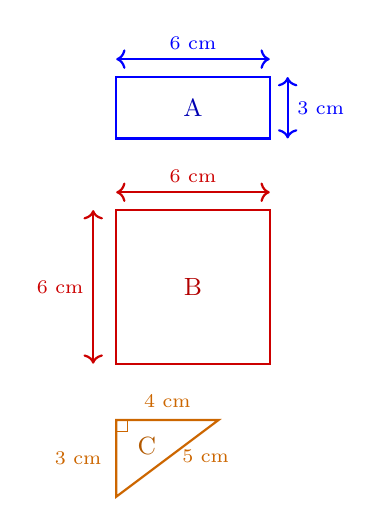
\begin{tikzpicture}[scale=0.65]

  \draw[thick, blue] (0,9.5) rectangle (3,8.3);
  \draw[blue, thick, <->] (0,9.85) -- (3,9.85);
  \node[blue, above] at (1.5,9.85) {\scriptsize 6 cm};
  \draw[blue, thick, <->] (3.35,8.3) -- (3.35,9.5);
  \node[blue, right] at (3.35,8.9) {\scriptsize 3 cm};
  \node[blue!70!black] at (1.5,8.9) {\small A};

  \draw[thick, red!80!black] (0,6.9) rectangle (3,3.9);
  \draw[red!80!black, thick, <->] (0,7.25) -- (3,7.25);
  \node[red!80!black, above] at (1.5,7.25) {\scriptsize 6 cm};
  \draw[red!80!black, thick, <->] (-0.45,3.9) -- (-0.45,6.9);
  \node[red!80!black, left] at (-0.45,5.4) {\scriptsize 6 cm};
  \node[red!70!black] at (1.5,5.4) {\small B};

  \draw[thick, orange!80!black] (0,2.8) -- (2,2.8) -- (0,1.3) -- cycle;
  \draw[orange!80!black] (0.22,2.8) -- (0.22,2.58) -- (0,2.58);
  \node[orange!80!black, above] at (1.0,2.85) {\scriptsize 4 cm};
  \node[orange!80!black, left] at (-0.1,2.05) {\scriptsize 3 cm};
  \node[orange!80!black, right] at (1.1,2.1) {\scriptsize 5 cm};
  \node[orange!70!black] at (0.6,2.3) {\small C};

\end{tikzpicture}
\end{center}

\column{0.62\textwidth}
\small
\begin{enumerate}
  \item \ealpara{Oblicz.}{$6 \times 3 =$ \ashowq{$18$}}
  \item \ealpara{Oblicz.}{$\frac{3}{24} + \frac{5}{24} =$ \ashowq{$\frac{1}{3}$}}
  \item \ealpara{Oblicz.}{$\tfrac{1}{2} \times 4 \times 3 =$ \ashowq{$6$}}
  \item \ealpara{Oblicz.}{$-3 \times -2 =$ \ashowq{$6$}}
  \item \ealpara{Znajdź \ealkeytr{średnią} z liczb $8,\ 14,\ 20$.}{Find the \ealkey{mean} of $\ 8,\ 14,\ 20$. \ashow{$14$}}
  \item \ealpara{Jakim \ealkeytr{ułamkiem} liczby $60$ jest $6$? \ealkeytr{Uprość} całkowicie.}{What \ealkey{fraction} of $60$ is $6$?\quad \ealkey{Simplify} fully. \ashow{$\frac{1}{10}$}}
\end{enumerate}

\vspace{0.5em}

\begin{enumerate}
  \setcounter{enumi}{6}
  \item \ealpara{Znajdź \ealkeytr{pole} każdej z figur A, B i C.}{Find the \ealkey{area} of each shape A, B and C. \ablank{$A=18$},\ \ablank{$B=36$},\ \ablank{$C=6$}.}
  \item \ealpara{Znajdź \ealkeytr{obwód} każdej z figur A, B i C.}{Find the \ealkey{perimeter} of each shape A, B and C. \ablank{$A=18$},\ \ablank{$B=24$},\ \ablank{$C=12$}.}
  \item \ealpara{Znajdź \ealkeytr{średnią} z \ealkeytr{pól} trzech figur.}{Find the \ealkey{mean} \ealkey{area} of the three shapes. \ablank{$20$}.}
  \item \ealpara{Znajdź \ealkeytr{średnią} z \ealkeytr{obwodów} trzech figur.}{Find the \ealkey{mean} \ealkey{perimeter} of the three shapes. \ablank{$18$}.}
  \item \ealpara{Jakim \ealkeytr{ułamkiem} całkowitego \ealkeytr{pola} jest figura C?}{What \ealkey{fraction} of the total \ealkey{area} does shape C make up? \ablank{$\frac{6}{60}=\frac{1}{10}$}.}
\end{enumerate}

\end{columns}
\end{frame}

%------------------------------------------------
% SLIDE 2: Areas, Perimeters, Mean & Fractions
%------------------------------------------------
\begin{frame}{Starter}

\begin{columns}

\column{0.38\textwidth}
\begin{center}
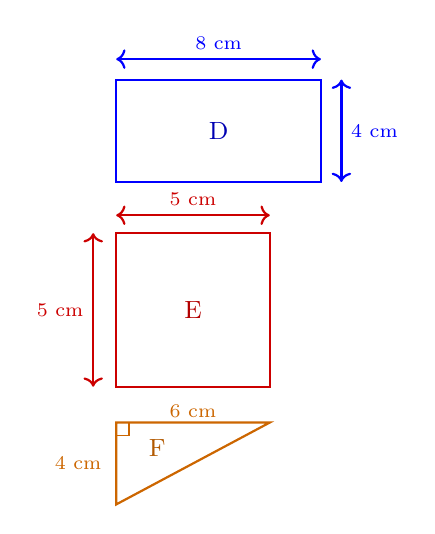
\begin{tikzpicture}[scale=0.65]

  \draw[thick, blue] (0,9.5) rectangle (4,7.5);
  \draw[blue, thick, <->] (0,9.9) -- (4,9.9);
  \node[blue, above] at (2,9.9) {\scriptsize 8 cm};
  \draw[blue, thick, <->] (4.4,7.5) -- (4.4,9.5);
  \node[blue, right] at (4.4,8.5) {\scriptsize 4 cm};
  \node[blue!70!black] at (2,8.5) {\small D};

  \draw[thick, red!80!black] (0,6.5) rectangle (3,3.5);
  \draw[red!80!black, thick, <->] (0,6.85) -- (3,6.85);
  \node[red!80!black, above] at (1.5,6.85) {\scriptsize 5 cm};
  \draw[red!80!black, thick, <->] (-0.45,3.5) -- (-0.45,6.5);
  \node[red!80!black, left] at (-0.45,5) {\scriptsize 5 cm};
  \node[red!70!black] at (1.5,5) {\small E};

  \draw[thick, orange!80!black] (0,2.8) -- (3,2.8) -- (0,1.2) -- cycle;
  \draw[orange!80!black] (0.25,2.8) -- (0.25,2.55) -- (0,2.55);
  \node[orange!80!black, above] at (1.5,2.7) {\scriptsize 6 cm};
  \node[orange!80!black, left] at (-0.1,2.0) {\scriptsize 4 cm};
  \node[orange!70!black] at (0.8,2.3) {\small F};

\end{tikzpicture}
\end{center}

\column{0.62\textwidth}
\small
\begin{enumerate}
  \item \ealpara{Oblicz.}{$8 \times 4 =$ \ashowq{$32$}}
  \item \ealpara{Oblicz.}{$\frac{7}{20} + \frac{9}{20} =$ \ashowq{$\frac{4}{5}$}}
  \item \ealpara{Oblicz.}{$\tfrac{1}{2} \times 6 \times 4 =$ \ashowq{$12$}}
  \item \ealpara{Oblicz.}{$-5 \times 4 =$ \ashowq{$-20$}}
  \item \ealpara{Znajdź \ealkeytr{średnią} z liczb $6,\ 12,\ 18$.}{Find the \ealkey{mean} of $\ 6,\ 12,\ 18$. \ashow{$12$}}
  \item \ealpara{Jakim \ealkeytr{ułamkiem} liczby $80$ jest $12$? \ealkeytr{Uprość} całkowicie.}{What \ealkey{fraction} of $80$ is $12$?\quad \ealkey{Simplify} fully. \ashow{$\frac{3}{20}$}}
\end{enumerate}

\vspace{0.5em}

\begin{enumerate}
  \setcounter{enumi}{6}
  \item \ealpara{Znajdź \ealkeytr{pole} każdej z figur D, E i F.}{Find the \ealkey{area} of each shape D, E and F. \ablank{$D=32$},\ \ablank{$E=25$},\ \ablank{$F=12$}.}
  \item \ealpara{Znajdź \ealkeytr{obwód} każdej z figur D, E i F.}{Find the \ealkey{perimeter} of each shape D, E and F. \ablank{$D=24$},\ \ablank{$E=20$},\ \ablank{$F=10+2\sqrt{13}$}.}
  \item \ealpara{Znajdź \ealkeytr{średnią} z \ealkeytr{pól} trzech figur.}{Find the \ealkey{mean} \ealkey{area} of the three shapes. \ablank{$23$}.}
  \item \ealpara{Znajdź \ealkeytr{średnią} z \ealkeytr{obwodów} trzech figur.}{Find the \ealkey{mean} \ealkey{perimeter} of the three shapes. \ablank{$\frac{54+2\sqrt{13}}{3}$}.}
  \item \ealpara{Jakim \ealkeytr{ułamkiem} całkowitego \ealkeytr{pola} jest figura F?}{What \ealkey{fraction} of the total \ealkey{area} does shape F make up? \ablank{$\frac{12}{69}=\frac{4}{23}$}.}
\end{enumerate}

\end{columns}
\end{frame}

\end{document}